% Created 2023-10-11 Wed 09:44
% Intended LaTeX compiler: pdflatex
\documentclass[smaller]{beamer}\usepackage{listings}
\usepackage{color}
\usepackage{amsmath}
\usepackage{array}
\usepackage[T1]{fontenc}
\usepackage{natbib}
\lstset{
keywordstyle=\color{blue},
commentstyle=\color{red},stringstyle=\color[rgb]{0,.5,0},
literate={~}{$\sim$}{1},
basicstyle=\ttfamily\small,
columns=fullflexible,
breaklines=true,
breakatwhitespace=false,
numbers=left,
numberstyle=\ttfamily\tiny\color{gray},
stepnumber=1,
numbersep=10pt,
backgroundcolor=\color{white},
tabsize=4,
keepspaces=true,
showspaces=false,
showstringspaces=false,
xleftmargin=.23in,
frame=single,
basewidth={0.5em,0.4em},
}
\usepackage{natbib, dsfont, pgfpages, tikz,amssymb, amsmath,xcolor}
\bibliographystyle{abbrvnat}
% New operators and commands
\newcommand{\Z}{\mathbb{Z}}
\newcommand{\Q}{\mathbb{Q}}
\newcommand{\R}{\mathbb{R}}
\newcommand{\N}{\mathbb{N}}
\newcommand{\C}{\mathbb{C}}
\renewcommand{\S}{\mathbb{S}}
\newcommand{\blank}{\makebox[1ex]{\textbf{$\cdot$}}}
\newcommand\independent{\protect\mathpalette{\protect\independenT}{\perp}}
\def\independenT#1#2{\mathrel{\rlap{$#1#2$}\mkern2mu{#1#2}}}
\renewcommand{\phi}{\varphi}
\renewcommand{\epsilon}{\varepsilon}
\newcommand*\diff{\mathop{}\!\mathrm{d}}
\newcommand{\weakly}{\rightsquigarrow}
\newcommand\smallO{
  \mathchoice
    {{\scriptstyle\mathcal{O}}}% \displaystyle
    {{\scriptstyle\mathcal{O}}}% \textstyle
    {{\scriptscriptstyle\mathcal{O}}}% \scriptstyle
    {\scalebox{.6}{$\scriptscriptstyle\mathcal{O}$}}%\scriptscriptstyle
}
\newcommand{\midd}{\; \middle|\;}
\newcommand{\1}{\mathds{1}}
\usepackage{ifthen} %% Empirical process with default argument
% \newcommand{\G}[1][]{%
%    \ifthenelse{ \equal{#1}{} }
%       {\ensuremath{\mathbb{G}_n}}
%       {\ensuremath{\mathbb{G}_{#1}}}
% }
% New version:
\newcommand{\G}[2][n]{
{\ensuremath{\mathbb{G}_{#1}}{\left[#2\right]}}
}
\DeclareMathOperator*{\argmin}{\arg\!\min}

% New operators for consistent notation
\newcommand{\V}{\mathrm{Var}} % variance
\newcommand{\measure}[1]{\mathrm{{#1}}} % measure
% \newcommand{\measure}[1]{\textnormal{\textbf{{#1}}}} % measure
\newcommand{\m}[1]{\measure{#1}} % measure shortcut
\newcommand{\eqd}{\stackrel{d}{=}} % equality in distribution
\newcommand{\arrow}[1]{\xrightarrow{\; {#1} \;}}
\newcommand{\arrowP}{\xrightarrow{\; \m{P} \;}} % convergence in probability
\newcommand{\leb}{\lambda} % the Lebesgue measure
\newcommand{\T}{\top} % transpose
\newcommand{\KL}{\ensuremath{D_{\mathrm{KL}}}}

\usepackage{xargs}
% Make it easy to change counterfactual notation:
\newcommandx{\cf}[4][3={}, 4={}]{
  % \ifthenelse{ \equal{#4}{} }
  % {{#1^{#2}}(#3)}
  {\ifthenelse{ \equal{#3}{} }
    {{#1^{#2}}_{#4}}
    {{#1^{#2}}_{#4}(#3)}}
}

% Easily change notation:
\DeclareMathOperator{\TT}{\Psi} % target parameter
\newcommand{\lp}{\mathcal{L}_{\P}^2} % shortcut for lp2 space
\newcommand{\empmeas}{\hat{\mathbb{P}}_n} % empirical measure
\DeclareMathOperator{\E}{\mathbb{E}} % expectation
\renewcommand{\P}{\m{P}} % probability
\newcommand{\ic}{\mathrm{IF}} % influence curve
\definecolor{bblue}{rgb}{0.2,0.2,0.7}
\usepackage{prodint}
\setbeamertemplate{footline}[frame number]
\beamertemplatenavigationsymbolsempty
\usepackage{appendixnumberbeamer}
\setbeamercolor{gray}{bg=white!90!black}
\setbeamertemplate{itemize items}{$\circ$}
\lstset{basicstyle=\ttfamily\footnotesize}

\renewcommand*\familydefault{\sfdefault}
\itemsep2pt
\usepackage[utf8]{inputenc}
\usepackage[T1]{fontenc}
\usepackage{graphicx}
\usepackage{longtable}
\usepackage{wrapfig}
\usepackage{rotating}
\usepackage[normalem]{ulem}
\usepackage{amsmath}
\usepackage{amssymb}
\usepackage{capt-of}
\usepackage{hyperref}
\usetheme{default}
\author{Anders Munch \newline \small joint work with Thomas Gerds}
\date{\today}
\title{The state learner \newline \normalsize a super learner for right-censored data}
\begin{document}

\maketitle
\begin{frame}{Outline}
\tableofcontents
\end{frame}

\section{Super learning with right-censored data}
\label{sec:org42945cb}
\begin{frame}[label={sec:orga8c5284}]{Super learning \small (aka cross-validation, stacked regression, \ldots{}\footnote{\cite{stone1974cross,geisser1975predictive,wolpert1992stacked,breiman1996stacked,van2007super}})}
\small

\color{bblue}Example: \color{black} Consider estimating a conditional mean \(f(x) = \E[Y \mid X=x]\) based on data \(\mathcal{D}_n = \{O_1, \dots, O_n\}\), where \(O_i = (X_i, Y_i)\) are iid.~observations.

\vfill

\begin{description}
\item[{Learner}] algorithm \(a\) that produces estimates, \(\mathcal{D}_n \mapsto
  a(\mathcal{D}_n) = \hat f_n\)
\item[{Library}] collection of learners, \(\mathcal{A} = \{a_1, a_2, \dots, a_M \}\)
\item[{Loss function}] \(L(a(\mathcal{D}_n), O)\), e.g., \(L(a(\mathcal{D}_n), O)
  = \{a(\mathcal{D}_n)(X) - Y\}^2\) \pause
\item[{Discrete SL}] \(\hat{a}_n = \argmin_{a\in\mathcal A}\hat{R}_n(a;
  L)\), where
\end{description}
\begin{equation*}
  \hat{R}_n(a; L) =
  \frac{1}{K}\sum_{k=1}^{K}
  \frac{1}{| \mathcal{D}_n^{k} |}\sum_{O_i \in \mathcal{D}_n^{k}}
  L
  {
    \left(
      a{ (\mathcal{D}_n^{-k})}
      , O_i
    \right)
  },
  \quad \text{with} \quad
  \mathcal{D}_n^{-k} = \mathcal{D}_n \setminus \mathcal{D}_n^{k}.
\end{equation*}


\vfill \pause

A super learner can be used for

\begin{itemize}
\item model selection and hyperparameter tuning
\item stand-alone prediction
\item nuisance parameter estimation (e.g., targeted learning of ATE)
\end{itemize}
\end{frame}

\begin{frame}[label={sec:org44e2829}]{Right-censored data}
\small

\begin{block}{Notation}
\begin{description}
\item[{\(X\)}] vector of baseline covariates
\item[{\(T\)}] time to event variable, \(T > 0\)
\item[{\(C\)}] censoring time, \(C > 0\)
\item[{\color{gray}\(\tilde T\)\color{black}}] censored time to event variable, \(\tilde T = \min(T, C)\)
\item[{\color{gray}\(\Delta\)\color{black}}] binary event indicator, \(\Delta =
  \1{\{T \leq C\}}\)
\item[{\color{gray}\(P\)\color{black}}] distribution of the observed data, \(O =
  (X, \tilde T, \Delta) \sim P\)
\item[{\(Q\)}] distribution of the data of interest \((X, T) \sim Q\)
\end{description}

\hfill

We use \color{bblue} \(\Lambda\) \color{black} and
\color{bblue}\(\Gamma\)\color{black}, respectively, to denote the conditional
cumulative hazard function for \(T\) and \(C\), i.e.,
\begin{equation*}
  \Lambda(\diff t \mid x) = Q(T \in \diff t \mid T \geq t, X=x).
\end{equation*}

We assume \(T \independent C \mid X\) and positivity, which implies that
\(\Lambda\) and \(\Gamma\) are identifiable from \(P\) on some time interval \([0,\tau]\).
\end{block}
\end{frame}

\begin{frame}[label={sec:org15dd7f4}]{Super learning with right-censored data}
\small

\begin{description}
\item[{\(P\)}] distribution of the observed data, \(O = (X, \tilde T, \Delta)
  \sim P\)
\item[{\(Q\)}] distribution of the data of interest \((X, T) \sim Q\)
\end{description}

\hfill

In a survival context, we have data \(\mathcal{D}_n = \{O_1, \dots, O_n\}\)
from \(P\), but we are interested in (a feature of) \(Q\), such as
\(\Lambda\).
\begin{equation*}
  \hat{R}_n(a; L) =
  \frac{1}{K}\sum_{k=1}^{K}
  \frac{1}{| \mathcal{D}_n^{k} |}\sum_{O_i \in \mathcal{D}_n^{k}}
  L
  {
    \left(
      a{ (\mathcal{D}_n^{-k})}
      , O_i
    \right)
  },
  \quad \text{with} \quad
  \mathcal{D}_n^{-k} = \mathcal{D}_n \setminus \mathcal{D}_n^{k}.
\end{equation*}

\pause

\begin{block}{The challenge of censoring}
\begin{description}
\item[{\(a{ (\mathcal{D}_n^{-k})}\)}] Many learners are available for this type of
data (e.g., semi-parametric Cox models, parametric survival models,
(stratified) Kaplan-Meier estimators, random survival forest) \(\checkmark\)
\item[{\(L(a{ (\mathcal{D}_n^{-k})} , O_i)\)}] How to evaluate the performance of
a learner trained in \(\mathcal{D}_n^{-k}\) in the hold-out data \(\mathcal{D}_n^{k}\)?
\end{description}
\end{block}
\end{frame}

\section{Existing approaches}
\label{sec:orge484da6}
\begin{frame}[label={sec:orgd032728}]{Existing approaches}
\small
\begin{block}{\normalsize Negative log-likelihood loss function \footnotesize (e.g., \cite{polley2011-sl-cens})}
Requires discrete time or modeling a Lebesgue hazard function which is
incompatible with many common estimators in survival analysis (e.g.,
Kaplan-Meier, semi-parametric Cox models, and random survival forests).
\end{block}

\begin{block}{\normalsize Pseudo-observations \footnotesize (e.g., \cite{sachs2019ensemble})}
Requires pre-specification of an estimator of the censoring mechanism.
\end{block}

\begin{block}{\normalsize IPCW \footnotesize (e.g., \cite{hothorn2006survival,gonzalez2021stacked})}
Inverse probability of censoring weighted loss functions also require a
pre-specified censoring model.
\end{block}

\begin{block}{\normalsize Iterative IPCW \footnotesize (\cite{westling2021inference,han2021inverse})}
To avoid this, it has been suggested to iterate between estimation of \(\Lambda\)
and \(\Gamma\). No theoretical guarantees for this procedure.
\end{block}
\end{frame}

\section{Proposal: The state learner}
\label{sec:orgc39f725}
\begin{frame}[label={sec:org7f82c91}]{The observed multi-state system}
Modeling the conditional state-occupation probabilities of the \emph{observed} data.

\hfill

\begin{onlyenv}<1>
\begin{block}{\centering \color{white} \((X, T) \sim Q\)}
\begin{center}
\includegraphics[width=.9\linewidth]{/tmp/babel-U9iZC3/figure-hAFBVF.pdf}
\end{center}
\end{block}
\end{onlyenv}

\begin{onlyenv}<2>
\begin{block}{\centering \((X, T) \sim Q\)}
\begin{center}
\includegraphics[width=.9\linewidth]{/tmp/babel-U9iZC3/figure-0XpsvW.pdf}
\end{center}
\end{block}
\end{onlyenv}

\begin{onlyenv}<3>
\begin{block}{\centering \color{gray}\((X, \tilde T, \Delta) \sim P\)\color{black}}
\begin{center}
\includegraphics[width=.9\linewidth]{/tmp/babel-U9iZC3/figure-W7BHHF.pdf}
\end{center}
\end{block}
\end{onlyenv}
\end{frame}


\begin{frame}[label={sec:org7c21fec}]{Conditional state-occupation probabilities for observed data}
\small

Record the observed data as \( O = (X, \{\eta(t) : t \geq 0\}) \), where
\begin{equation*}
  \eta(t) = \1{\{\tilde{T} \leq t, \Delta = 1\}} + 2 \, \1{\{\tilde{T} \leq t,
    \Delta = 0\}}
  \in \{0, 1, 2\}.
\end{equation*}

Denote by
\begin{equation*}
  F(t, j, x) = P(\eta(t) = j \mid X=x), \quad \text{for all } t \geq 0,\; j
  \in \{0, 1, 2\}, \; x \in \R^d,
\end{equation*}
the conditional state-occupation probabilities for the observed data.

\vfill

\begin{columns}
\begin{column}{0.45\columnwidth}
\centering \color{bblue}\(O = (X, \tilde T , \Delta)\)\color{black} 

\begin{center}
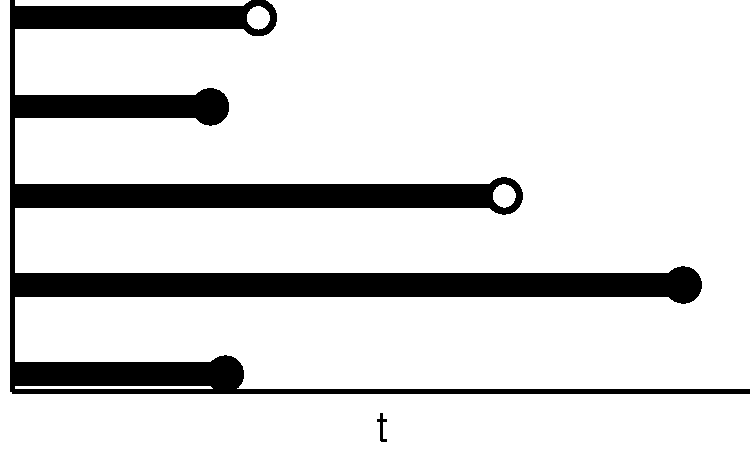
\includegraphics[width=0.9\textwidth]{./multi-state-data-1.pdf}
\end{center}
\end{column}

\begin{column}{0.45\columnwidth}
\centering \color{bblue}\(O = (X, \{\eta(t) : t \geq 0\})\)\color{black}

\begin{center}
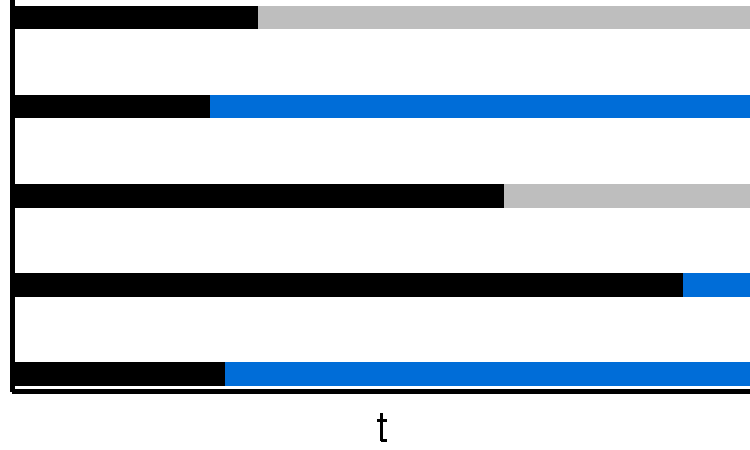
\includegraphics[width=0.9\textwidth]{./multi-state-data-3.pdf}
\end{center}
\end{column}
\end{columns}
\end{frame}

\begin{frame}[label={sec:org3b02a1b}]{The state learner}
\small

The state learner builds a super learner for the conditional state-occupation
probabilities,
\begin{equation*}
  F(t, j, x) = P(\eta(t) = j \mid X=x), \quad \text{for all } t \geq 0,\; j
  \in \{0, 1, 2\}, \; x \in \R^d.
\end{equation*}

\(F\) is a feature of the observed data distribution \(P\), so performance
can be evaluated directly as in a ``non-survival'' setting.

\vfill

We suggest to use the integrated Brier score
\( \bar{B}_{\tau}(F, O) = \int_0^{\tau} B_t(F, O) \diff t \), where
\begin{equation*}
  B_t(F, O) = \sum_{j=0}^{2} (F(t, j, X) - \eta(t))^2.
\end{equation*}

With this choice of loss function no modeling of Lebesgue hazards or densities
is required.
\end{frame}

\begin{frame}[label={sec:org57f8c50}]{Expressing \(F\) using \(\Lambda\) and \(\Gamma\)}
\small

\begin{equation*}
  F(t, j, x) = P(\eta(t) = j \mid X=x), \quad \text{for all } t \geq 0,\; j
  \in \{0, 1, 2\}, \; x \in \R^d
\end{equation*}
can be expressed (slightly informally) using $\Lambda$ and $\Gamma$,
\begin{equation*}
\begin{split}
F(t, 1, x)
& = P(\tilde{T} \leq t, \Delta=1 \mid X=x)
  = \int_0^t e^{-\Lambda(s \mid x) - \Gamma(s \mid x) }  \Lambda(\diff s \mid x),
\\
F(t, 2, x)
& = P(\tilde{T} \leq t, \Delta=0 \mid X=x)
  = \int_0^t e^{-\Lambda(s \mid x) - \Gamma(s \mid x) }  \Gamma(\diff s \mid x),
\\
F(t, 0, x)
&
  = P(\tilde{T} > t \mid X= x)
  = 1- F(t, 1, x) - F(t, 2, x).
\end{split}
\end{equation*}

\vfill

\begin{center}
\includegraphics[width=.9\linewidth]{/tmp/babel-U9iZC3/figure-wHmT7y.pdf}
\end{center}
\end{frame}

\begin{frame}[label={sec:org9195dc2}]{Constructing a library for learning \(F\)}
\small

Many learners for \(\Lambda\) (and \(\Gamma\)) are avalaible (Cox models, random
survival forests, etc.).

\vfill

Given libraries \( \mathcal{A} \) and \( \mathcal{B} \) for learning $\Lambda$
and $\Gamma$, respectively,  we construct the library
\begin{equation*}
  \mathcal{F}(\mathcal{A}, \mathcal{B})
  = \{ \phi_{a, b} : a \in \mathcal{A}, b \in \mathcal{B}\},
\end{equation*}
where
\begin{align*}
  \phi_{a, b}(\mathcal{D}_n)(t,1,x) &= \int_0^t e^{-a(\mathcal{D}_n)(s \mid
    x) -
    b(\mathcal{D}_n)(s \mid x) }  a(\mathcal{D}_n)(\diff s \mid x),
  \\
  & \dots 
\end{align*}

We evaluate performance of every
\( \phi_{a, b} \in \mathcal{F}(\mathcal{A}, \mathcal{B}) \) as
\begin{equation*}
  \hat{R}_n(\phi_{a, b}; \bar{B}_{\tau}) =
  \frac{1}{K}\sum_{k=1}^{K}
  \frac{1}{| \mathcal{D}_n^{k} |}\sum_{O_i \in \mathcal{D}_n^{k}}
  \int_0^{\tau} \sum_{j=0}^{2} 
  \left\{
    \phi_{a, b}(\mathcal{D}_n^{-k})(t,j, X_i) - \eta_i(t)
  \right\}^2 \diff t.
\end{equation*}
\end{frame}


\begin{frame}[label={sec:org78c70b6}]{Some theoretical results}
\small

\begin{block}{Finite sample guarantee}
Using results from \citep{van2003unicv,van2006oracle} we can establish a finite
sample oracle inequality for the state learner.

\hfill

This means that the state learner will perform almost as well as a so-called
``oracle'' which uses the unknown data-generating distribution to evaluate
performance of the learners.

\hfill
\end{block}

\begin{block}{Asymptotic consequence}
Let \(F_0\) denote the conditional state-occupation probability function
corresponding to the underlying data-generating distribution \(P_0\). If

\begin{itemize}
\item \(|\mathcal{F}(\mathcal{A}_n,\mathcal{B}_n)| = O(n^q)\), for some \(q \in
  \N\), and
\item the library contains a learner that converges to \(F_0\) at rate \(r_n\),
\end{itemize}

then the state learner converges to \(F_0\) at the same rate or at rate \(\log(n) r_n\).
\end{block}
\end{frame}


\begin{frame}[label={sec:org9906459},fragile]{Almost minimum viable product}
 \footnotesize

\lstset{language=r,label= ,caption= ,captionpos=b,numbers=none}
\begin{lstlisting}
head(use_dat, n=4)
\end{lstlisting}

\begin{verbatim}
       time status   logPSA stage ggtot      sDose hormones
1: 30.78737      0 1.791759   T1c     6  0.1663670       No
2: 28.69895      0 2.468100   T3c     9  0.1663670      Yes
3: 11.99158      0 3.086487   T1c     3 -0.9372808       No
4: 38.13053      1 2.890372   T1c     6 -0.9372808       No
\end{verbatim}


\lstset{language=r,label= ,caption= ,captionpos=b,numbers=none}
\begin{lstlisting}
library <- list(
  cox_lasso = list("GLMnet"),
  cox_elastic = list("GLMnet", alpha = 0.5),
  rf = list("rfsrc", ntree = 500))
fit_sl <- statelearner(
  list(cause1 = library, censor = library),
  data = use_dat, time = 36),
head(fit_sl, n=4)
\end{lstlisting}

\begin{verbatim}
        cause1 censor     loss         sd
1: cox_elastic     rf 7.034702 0.02159417
2: cox_elastic     rf 7.034812 0.02286074
3:   cox_lasso     rf 7.035051 0.02142064
4:   cox_lasso     rf 7.035231 0.02266556
\end{verbatim}
\end{frame}



\begin{frame}[label={sec:org1447ea9}]{Proof of concept -- simulation I}
\small

\begin{itemize}
\item Univariate \(X\)
\item Cox model and the Nelson-Aalen estimator in the libraries
\item Compare to IPCW weighted estimators using wrongly (IPCW(KM)) and correctly
(IPCW(Cox)) specified censoring models
\item Evaluate performance of survival predictions at fixed prediction horizon
\end{itemize}

\begin{center}
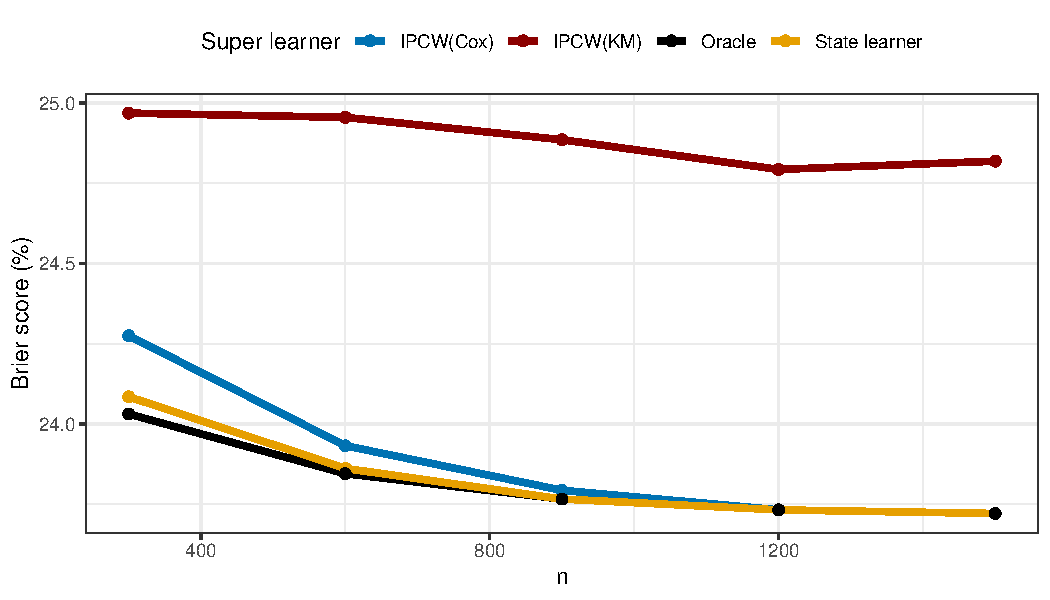
\includegraphics[width=.9\textwidth]{./ipcw-fail.pdf}
\end{center}
\end{frame}

\begin{frame}[label={sec:org531a91d}]{Proof of concept -- simulation II}
\small

\begin{itemize}
\item Multivariate \(X\)
\item Several strong learners: Cox models (various stratifications and splines),
penalized Cox models (lasso, ridge, elastic), random survival forest
\item Data generated according to a simulation of a prostate cancer study
\citep{kattan2000pretreatment,gerds2013estimating}.
\end{itemize}

\begin{center}
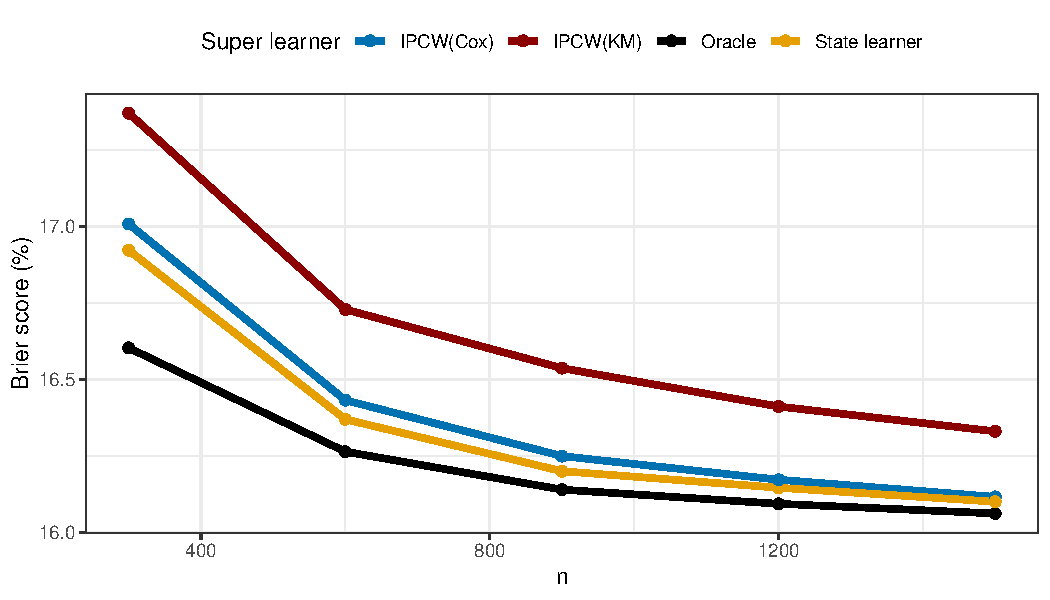
\includegraphics[width=.9\textwidth]{./zelefski-sim.pdf}
\end{center}
\end{frame}

\begin{frame}[label={sec:orge134f36}]{Competing risks}
\small

\begin{center}
\includegraphics[width=.9\linewidth]{/tmp/babel-U9iZC3/figure-jHSzxz.pdf}
\end{center}

\begin{equation*}
  \eta(t) = \1{\{\tilde{T} \leq t, \tilde{D} = 1\}} +
  2 \, \1{\{\tilde{T} \leq t, \tilde{D} = 2\}}
  +
  3 \, \1{\{\tilde{T} \leq t, \tilde{D} = 0\}}.
\end{equation*}
\begin{align*}
  F(t, 1, x)
  & = P(\tilde{T} \leq t, \tilde{D}=1 \mid X=x)
    = \int_0^t e^{-\Lambda_1(s \mid x) -\Lambda_2(s \mid x) - \Gamma(s \mid x) }  \Lambda_1(\diff s \mid x),
  \\
  & \dots
\end{align*}
\begin{equation*}
  \mathcal{F}(\mathcal{A}_1,\mathcal{A}_2, \mathcal{B})
  = \{ \phi_{a_1, a_2, b} : a_1 \in \mathcal{A}_1, a_2 \in \mathcal{A}_2, b \in \mathcal{B}\},
\end{equation*}
\end{frame}

\begin{frame}[label={sec:org27a14ae}]{Proof of concept -- some real data}
\small The real data considered in \citep{kattan2000pretreatment} included the
competing risk of death.

\begin{center}
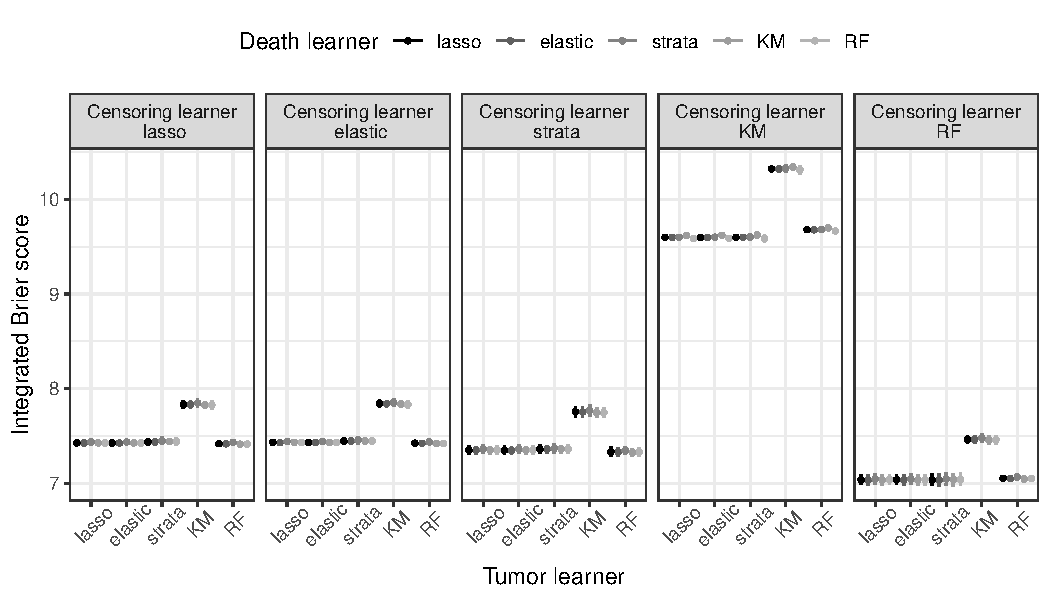
\includegraphics[width=1\textwidth]{./zelefski-real-data.pdf}
\end{center}
\end{frame}

\section{Discussion}
\label{sec:org8b38693}
\begin{frame}[label={sec:org92a75dd}]{Discussion}
\small

A clear limitation is that the function \(F\) is typically not a parameter of
interest.

\vfill

We can obtain a risk prediction model from the state learner using that
\begin{equation*}
  \Lambda(t \mid x) = \int_0^t \frac{F(\diff s, 1, x)}{F(s-, 0, x)} ,
  \quad \text{and} \quad
  S(t \mid x)
  % = Q(T > t \mid X=x)
  % = e^{\Lambda(t \mid x)}
  = \prodi_{s \leq t}(1- \Lambda(\diff s \mid x)).
\end{equation*}

However, the state learner does not evaluate the learners based on their risk
prediction performances but on how well a tuple \((\Lambda, \Gamma)\) of
learners jointly model the observed data.

\vfill

When estimating low-dimensional target parameter and the state learner is used
to estimate the nuisance parameters, this is probably less of a concern.

\vfill

Unclear if the state learner will respond well to positivity violations or not.
\end{frame}

\begin{frame}[label={sec:org5faf490}]{Conclusion}
\small

\begin{itemize}
\item To avoid the need to pre-specify a censoring model, we propose to use learners
for \(\Lambda\) and \(\Gamma\) to jointly model the observed data.
\item We select a tuple of learners \((\Lambda, \Gamma)\) that is jointly optimal
for predicting the states occupied by the observed data conditional on
baseline covariates.
\item We use the integrated Brier score to evaluate performance with
respect to the observed data distribution.
\item No need to model additional nuisance parameters to estimate performance in
hold-out samples.
\item No need to estimate Lebesgue densities or hazards.
\item Drawback is that the SL is tuned for the a feature of the observed
distribution \(P\) and not for a feature of \(Q\).
\end{itemize}

\vfill


\begin{block}{Questions, comments, suggestions?}
\vfill

\flushright Thank you for listening!
\end{block}
\end{frame}

\section*{References}
\label{sec:orgecdcc08}
\begin{frame}[label={sec:org8c9e969}]{References}
\tiny \bibliography{./latex-settings/default-bib.bib}
\end{frame}
\end{document}